% coding:utf-8

%FOSAET, a LaTeX-Code for a electrical summary of basic electronics
%Copyright (C) 2013, Daniel Winz, Ervin Mazlagic

%This program is free software; you can redistribute it and/or
%modify it under the terms of the GNU General Public License
%as published by the Free Software Foundation; either version 2
%of the License, or (at your option) any later version.

%This program is distributed in the hope that it will be useful,
%but WITHOUT ANY WARRANTY; without even the implied warranty of
%MERCHANTABILITY or FITNESS FOR A PARTICULAR PURPOSE.  See the
%GNU General Public License for more details.
%----------------------------------------

\subsection{Aktiver Hochpass 2. Ordnung}
\begin{figure}[h!]
	\centering
	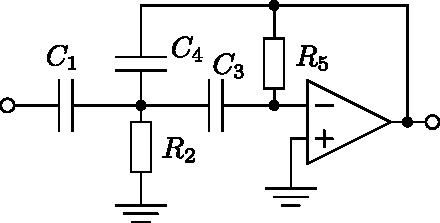
\includegraphics[scale=\schscale]{op_hp_o2.pdf}
	\caption{Aktiver Hochpass 2. Ordnung}
	\label{sch:op-hp-o2}
\end{figure}
\[ \frac{-H \cdot s^2}{s^2 + \alpha \cdot \omega_0 \cdot s + {\omega_0}^2} \]
\[ \frac{V_{out}}{V_{in}} = \frac{- s^2 \cdot \frac{C_1}{C_4}}
{s^2 + s \cdot \frac{C_1 + C_3 + C_4}{C_3 \cdot C_4 \cdot R_5} 
+ \frac{1}{R_2 \cdot R_5 \cdot C_3 \cdot C_4}} \]
\[ \alpha = \frac{1}{Q} \]
\subsubsection{Dimensionierung}
\[ C_1 \text{ wählen} \]
\[ k = 2 \cdot \pi \cdot f_0 \cdot C_1 \]
\[ C_3 = C_1 \]
\[ C_4 = \frac{C_1}{H} \]
\[ R_2 = \frac{\alpha}{k \cdot \left(2 + \frac{1}{H}\right)} 
= \frac{1}{Q \cdot k \cdot \left(2 + \frac{1}{H}\right)} \]
\[ R_5 = \frac{H \cdot \left(2 + \frac{1}{H}\right)}{\alpha \cdot k} 
= \frac{Q \cdot H \cdot \left(2 + \frac{1}{H}\right)}{k} \]
